% TRR_latex_guidelines.tex V1.00, 31 August 2020

\documentclass[times]{TRR}

\usepackage{moreverb,url}
\graphicspath{{images}}
%\usepackage[numbers]{natbib}
\usepackage[table]{xcolor}
\usepackage{multirow}

\usepackage[colorlinks,bookmarksopen,bookmarksnumbered,citecolor=red,urlcolor=red]{hyperref}

\newcommand\BibTeX{{\rmfamily B\kern-.05em \textsc{i\kern-.025em b}\kern-.08em
T\kern-.1667em\lower.7ex\hbox{E}\kern-.125emX}}

\def\volumeyear{2022}

\begin{document}

\runninghead{Han et al.}

\title{Modeling system-wide urban rail transit energy consumption: A case study of Boston}

\author{Zhuo Han\affilnum{1}, Eric Gonzales\affilnum{1}, Eleni Christofa\affilnum{1}, Jimi Oke\affilnum{1}}

\affiliation{
\affilnum{1}Department of Civil and Environmental Engineering, University of Massachusetts Amherst, MA 01003, United States}

\corrauth{Zhuo Han, zhuohan@umass.edu}

\begin{abstract}
Rapid transit systems are critical components of public transportation networks in urban areas both in terms of their impact on person mobility but also on monetary, energy, and environmental costs associated with their operations. In order to facilitate effective planning for current and future needs, a framework is required that not only provides important consumption metrics but also explains the various contributors to energy consumption and their interactions. This paper presents a model that utilized operational and ridership data for the Massachusetts Bay Transportation Authority's rapid transit system, as well as  ambient temperature, to accurately predict system-wide electricity consumption. We estimated linear regression and random forest models, which explained 93\% and 95\% of the variance in the data set, respectively.  The models were trained with data from 2019 and tested with data from 2020.  The linear regression model provided predictions with an RMSE of 2.7 MWh and MAPE of 4.68\%, and the random forest model resulted in an RMSE of 2.94 MWh and MAPE of 5.01\%. We also investigate the impacts of COVID-19 on the transit system by exploring the effects on ridership, energy consumption, cost and train movement metrics before and during the pandemic. We find that the models are robust and perform well even with the significant disruptions associated with the  pandemic.\\

\textit{Keywords}: rail transit, energy, system modeling, sustainability, COVID-19
\end{abstract}

\maketitle

\section{Introduction}
Urban rapid transit systems typically use electric trains to move heavy and light rail vehicles with high passenger capacity.  Large transit systems use hundreds of gigawatt-hours of electricity each year to carry millions of people.  The accurate prediction of the energy consumption of rail vehicles is thus important for planning operations, managing a fleet, making energy purchasing agreements, and understanding the environmental impacts of a system. Although it is well known that train acceleration and speed, ridership, weather conditions, and several other factors can impact the energy consumption of trains, the individual contributions of each of these factors is not fully understood.  Therefore, a model that accurately predicts the energy consumption of rapid transit systems would be valuable for managing transit operations in order to limit energy-related expenditures while serving passenger needs.


This paper addresses the gap in understanding the factors that contribute to energy consumption in an urban rapid transit system and how they interact. To this end, this research investigates the system-level relationship between energy consumption and train movement in an urban rapid transit system via an interpretable modeling framework.
During the course of the study, the COVID-19 pandemic had a profound impact on rapid transit ridership and operations, which led to greater variation in ridership and train operations than would normally be expected. These changes prompted the added objective of evaluating the impact of operations during the pandemic on system-wide energy consumption.

As a case in point, the Massachusetts Bay Transportation Authority (MBTA) operates the public transportation network that serves the Boston metropolitan area---the fourth busiest in the United States by passenger ridership \cite{aptaadmin2021ridership}. It comprises of a light rail line (Green Line) and three heavy rail lines (Red, Orange, and Blue) as shown on the system map \autoref{fig1}.  The MBTA currently has meters at electric substations throughout the system but no direct measurements of electricity consumption by trains. The energy consumption of the rapid transit system is significant, with the MBTA spending an average of \$38 million on 422 GWh of electricity for the system per year. This includes demand for vehicle traction power, signal systems, and station operations. 

\begin{figure*}[h!]
    \centering
    \includegraphics[width=.7\textwidth]{Figure_1_subway_map_may_2021_GLX_stops.pdf}
    \caption{Schematic map of the rapid transit network of the Massachusetts Bay Transportation Authority. The lines considered for this study are: Red, Blue, Orange (heavy rail) and Green (light rail).
    Image source: \url{https://www.mbta.com/schedules/subway}
    }
    \label{fig1}
\end{figure*}


This paper is organized into three main parts.  First, an exploratory analysis of the available energy consumption and train operations data from the MBTA provides general insights about temporal trends and the relationships between the data.  An automated process is developed to construct detailed trajectories for each vehicle’s movement through the system, including calculation of speed and acceleration, which are important determinants of the energy required for tractive power. Second, a linear regression model and a Random Forests model are developed and estimated to relate explanatory factors to the system-wide energy consumption of the MBTA rapid transit system. These models are analyzed to identify the factors with the strongest effect on energy consumption.  Third, the performance of the models is tested with training data from 2019. The models are then used to make predictions on observations from 2020.  The performance is particularly revealing, because the COVID-19 pandemic led to significant reductions in rapid transit ridership and train operations, which tests the ability of the model to accurately capture these effects on energy consumption.


\section{Literature Review} 
Urban rail transit is most promising as a sustainable mode of transportation, as it contributes the least to transportation energy demand. 
Historically, several efforts have aimed to accurately model the energy consumption of train vehicles and proposed various approaches for reducing consumption.
Notably, \citeauthor{wang2017electric} \cite{wang2017electric} created a train energy framework, which takes instantaneous regenerative braking efficiency into account, and demonstrated that a 20\% reduction in energy consumption was possible in the Chicago network. Others have developed simulation, optimization, or machine learning approaches to find energy reduction pathways \cite{higuera2016energy, mao2018modeling,ruigang2017simulation, modi2020estimation, malikopoulos2012optimization, oettich2004improvements, li2018calculation}. In all of these instances, energy reductions were achieved by solving for optimal vehicle trajectory patterns or schedule changes. In real-world cases, however, these solutions are not often feasible to implement.

A few other researchers have attempted to pinpoint other sources of transit system-wide energy consumption besides train operations themselves. For instance, \cite{wang2020rail} demonstrated that lighting systems in underground stations are a significant contributor to overall energy consumption. \citeauthor{gonzalez-gil2014systems} \cite{gonzalez-gil2014systems} showed that energy gains of over 25\% are possible via a combination of efficient driving strategies, smart metering, and power management, along with small-scale renewable generation. \citeauthor{leung2013estimation} \cite{leung2013estimation} estimated a model that indicated station design and weather as important factors for energy consumption in a rail transit system.

The physical characteristics of railroads and train routes also have significant effects on energy consumption. Some research efforts thus proposed models for selecting the optimal vertical alignment or transit route design in order to reduce  system energy usage and associated costs. \citeauthor{kang2014rail}  \cite{kang2014rail} developed an optimization model  for choosing the best train route. The selected route not only maximized the net benefits but also satisfied geometric design constraints.  Comparisons and analysis of different vertical alignment designs have been conducted to find the most energy-efficient solution for railroads \cite{kim2019vertical,kim2013comparison} and highways \cite{kang2013new}. In this study, however, the network geometry is fixed. Thus, the model for system-wide energy consumption is estimated based on the MBTA's existing infrastructure.


These developments notwithstanding, there remains a gap in the literature on simple system-wide models that are not only highly interpretable and but also high-performing in their predictive capability. Such models can be extremely useful for planners in understanding how various aspects of the transit system impact energy consumption, beyond train movements, as well as in providing practical pathways to reduce energy consumption, and consequently, costs, both of which are of great importance. The research presented in this paper addresses this gap by estimating models based on the rail network that serves the Boston area. We demonstrate that our approach is readily deployable on transit systems in order to yield similarly useful insights.


\section{Data}
 The goal of the study is to determine the key factors affecting system-wide energy consumption via an interpretable model that can also reliably predict electricity consumption based on readily observable factors. Thus, we use data obtained for the MBTA rapid transit system in Boston, Massachusetts, and surrounding communities (\autoref{fig1}).  The following subsections provide descriptions of the data on energy consumption, energy costs, ridership, train movements, and weather, all of which were used in the modeling process.

\subsection{Energy consumption}
Energy consumption data from 2008 to 2020 was extracted from spreadsheets provided by MBTA.  Monthly energy use from these years is shown in \autoref{fig2} via a boxplot. This figure reveals that the greatest monthly energy consumption occurs consistently during the winter months, presumably due to heating needs. Peak usage is observed in January (average of 43 GWh). From April through November, energy consumption is visibly lower, presumably due to reduced third rail heating needs. A smaller peak, however, is observed in July, which is typically the hottest month of the year during which the demand for air conditioning is greatest. Thus, weather appears to be a significant explanatory variable for energy consumption.

\begin{figure*}[htbp]
    \centering
    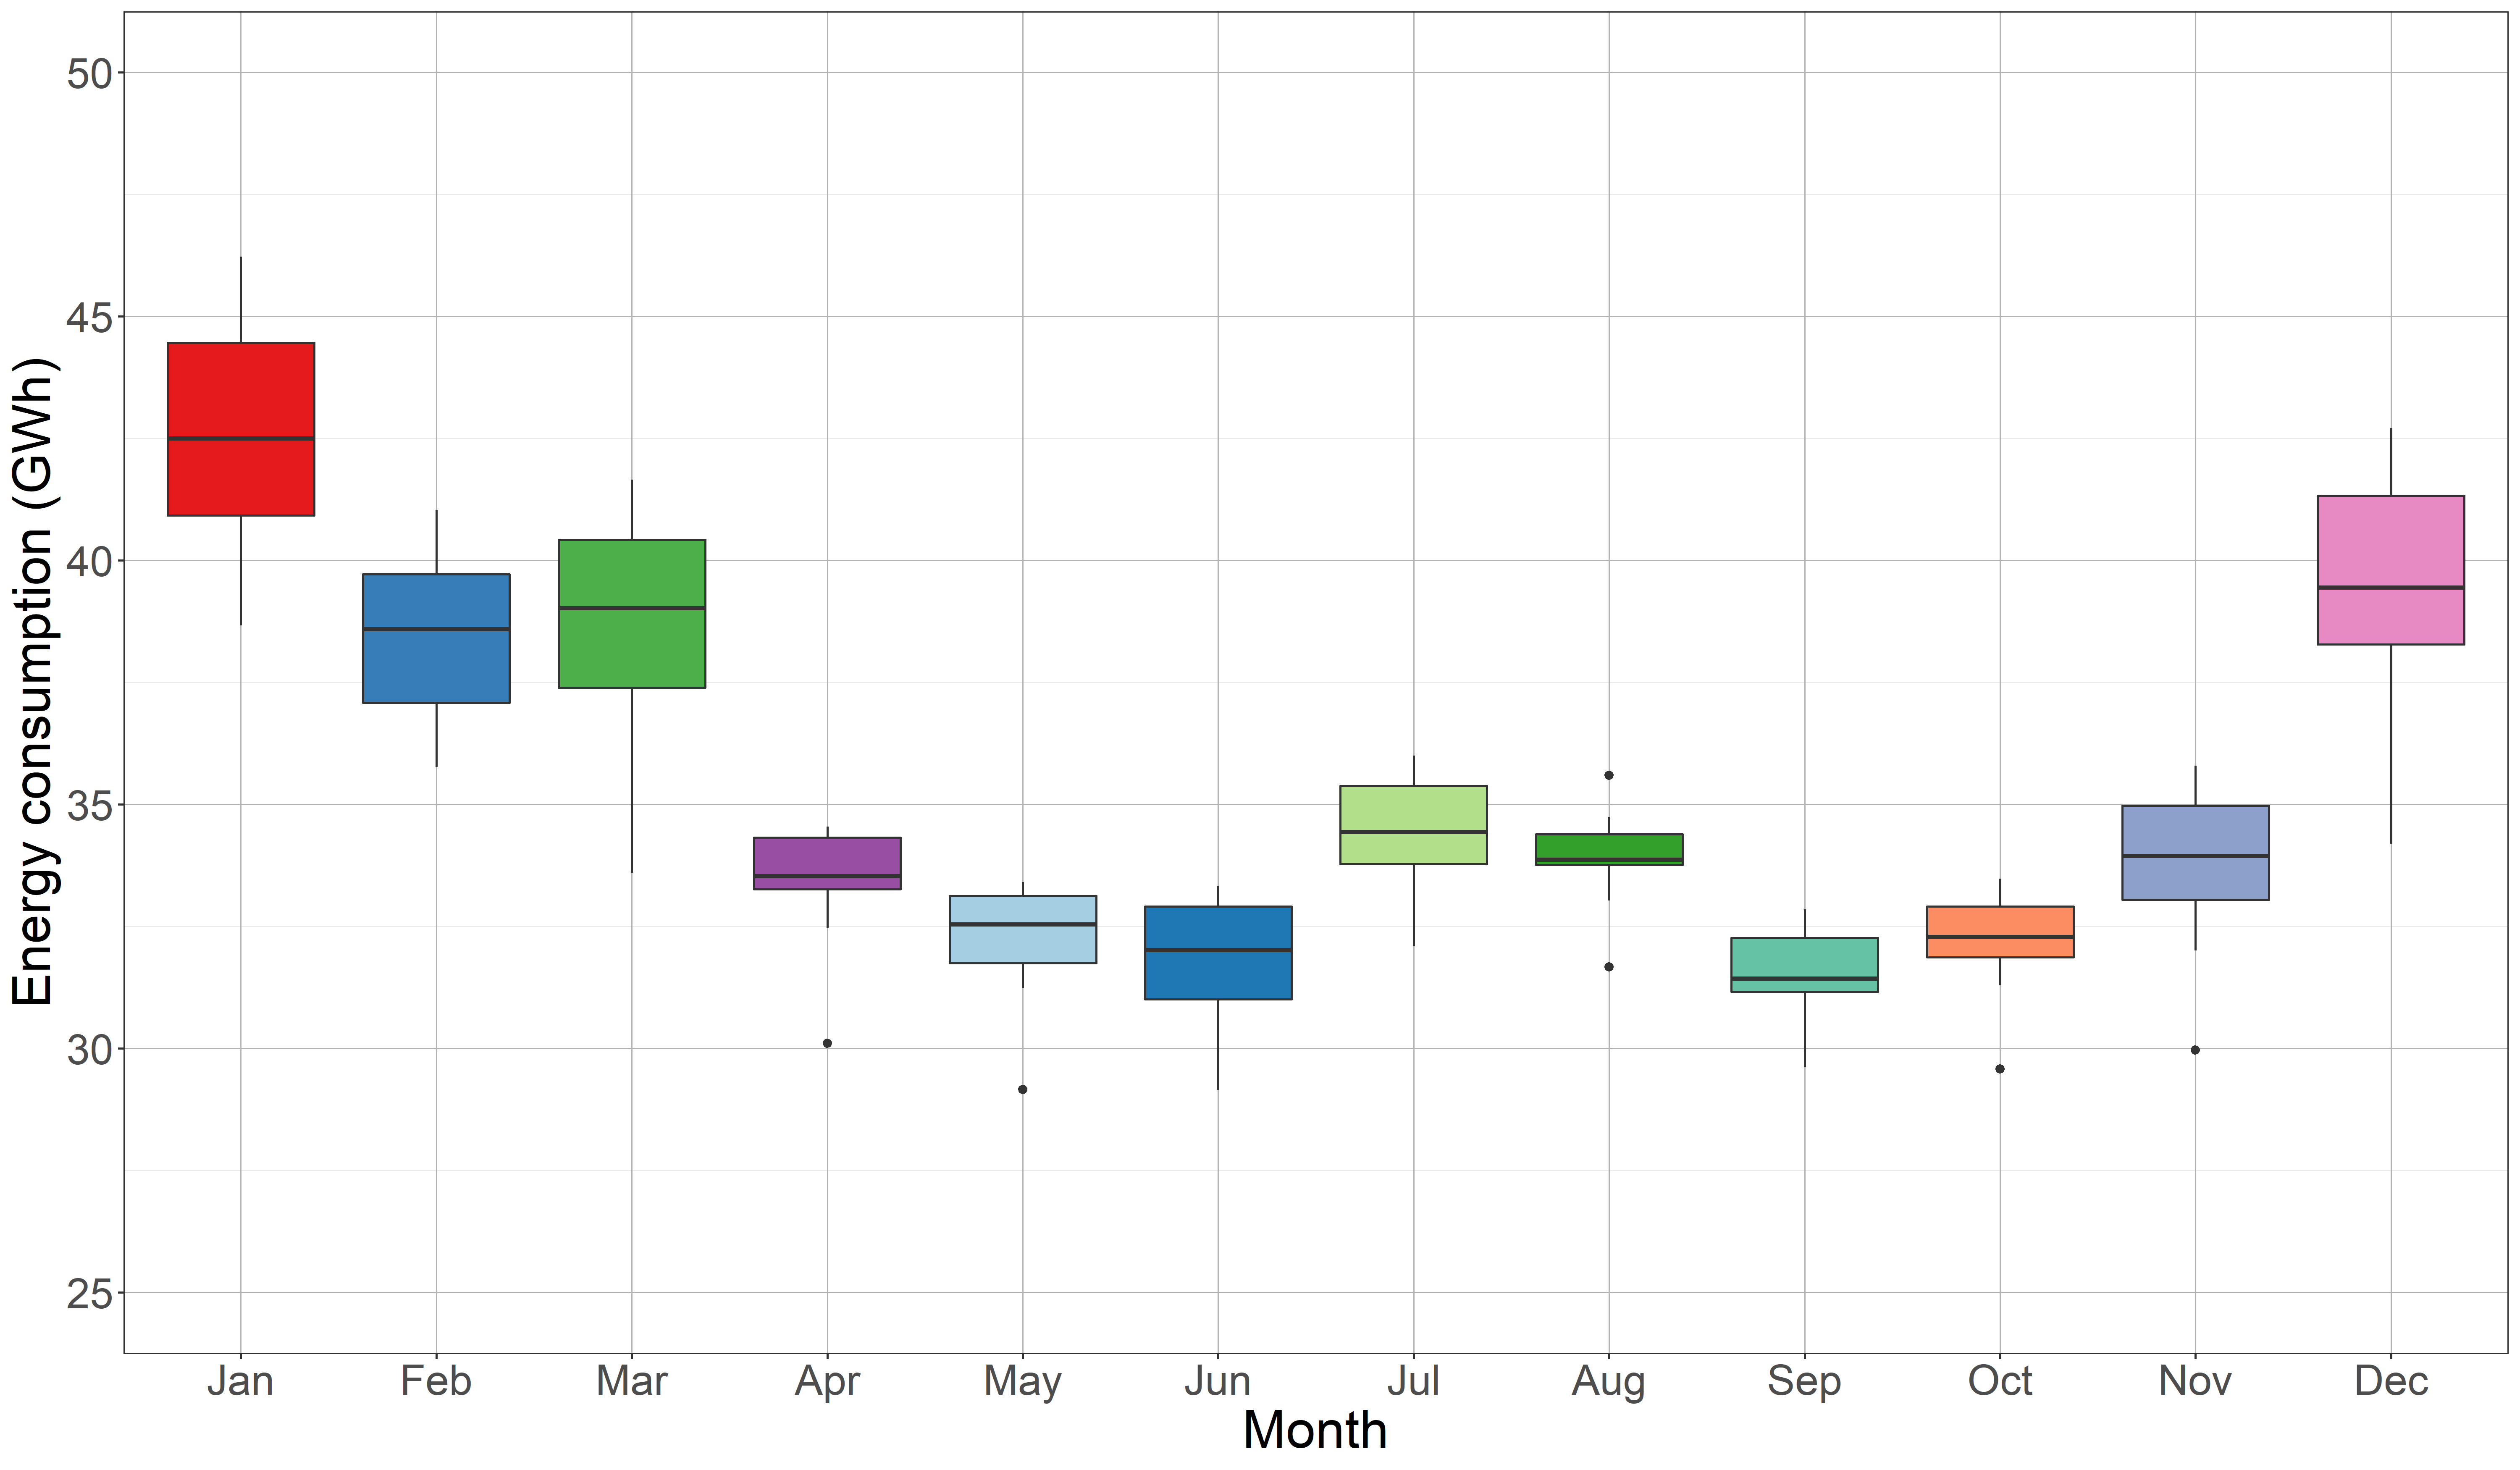
\includegraphics[width=.8\textwidth]{Figure_2_Month_box_plot.png}%Month box plot.png
    \caption{Boxplot of MBTA rapid transit monthly energy usage, 2008--2020. The height of each box indicates the interquartile range of observations in that month. Horizontal lines in the boxes indicate the median.}
    \label{fig2}
\end{figure*}

The hourly energy distribution, also based on observations from 2008 to 2020, is shown in \autoref{fig3}. The boxplot indicates that the peak consumption period occurs from 7 to 9 AM and from 4 to 6 PM, which are the hours associated with the most frequent train operations. For reference, the average hourly peak energy consumption in 2019 was 53 MWh and average overnight hourly energy peak was 75 MWh. The ``overnight'' period corresponds to the hours during which there is minimal train movement and no ridership, as the MBTA rapid transit system closes from a period after midnight until about 5 AM. The lowest energy consumption occurs between 2 and 4 AM, when the system is closed, yet there is a baseline average energy consumption of 34 MWh during this period. The overall average hourly energy consumption from 2008 to 2020 is 48 MWh. 

\begin{figure*}[htbp]
    \centering
    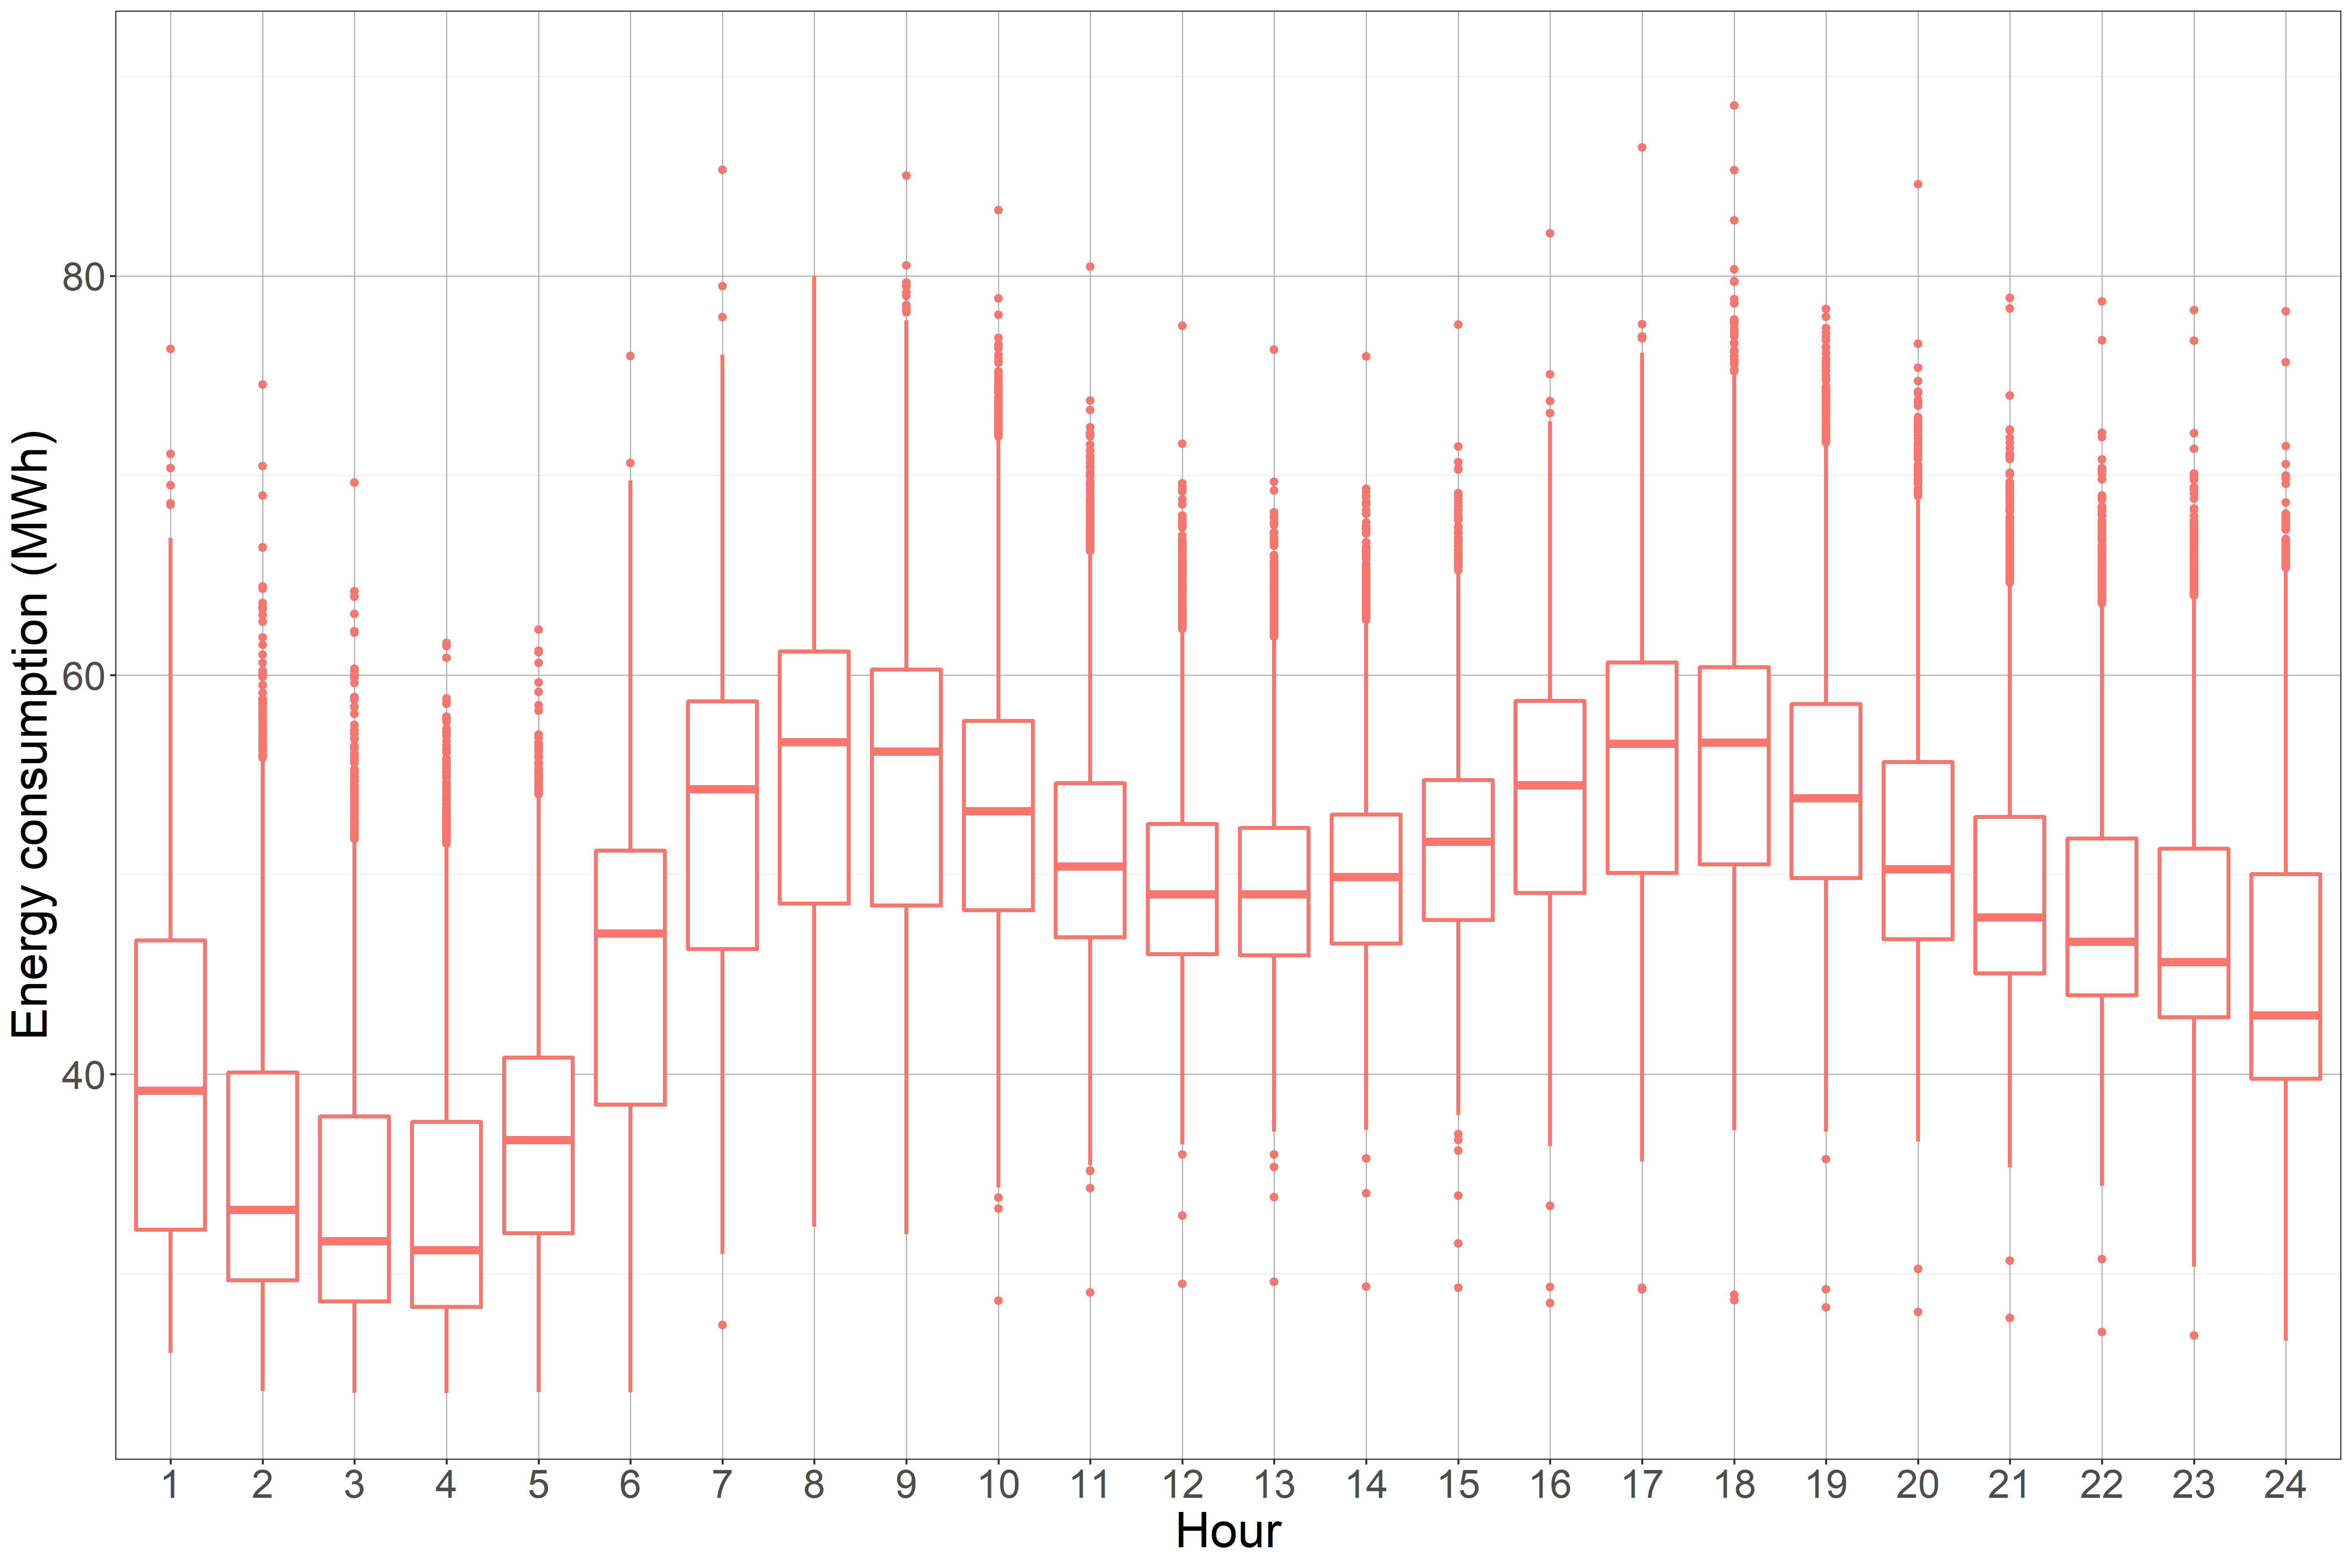
\includegraphics[width=.8\textwidth]{Figure_3_Hourly_box_plot.png}
    \caption{Boxplot of MBTA rapid transit hourly energy consumption }
    \label{fig3}
\end{figure*}

The time series of hourly energy consumption for the years 2019 and 2020 is shown in \autoref{fig4} (a).  Energy consumption declined sharply in March 2020, coinciding with the beginning of the pandemic and the associated lockdown policies.

\begin{figure*}[ht!]
    \centering
    \includegraphics[width=.8\textwidth]{Figure_4_Time_series.png}
    \caption{Time series plots of energy, ridership, vehicle-miles, vehicle-hours, and operating trains (at the hour resolution) and average daily temperature, from January 2019 through December 2020 for the MBTA rapid transit system.}
    \label{fig4}
\end{figure*}

\subsection{Ridership}
System-wide hourly ridership data were obtained from the MBTA Research Database for 2019 and 2020. The time series is shown in \autoref{fig4} (b).  The ridership is sourced from farecard tap-in data that logs the location and time that each passenger enters the system.  These data provide reliable counts of total ridership in aggregate. Since the MBTA's rapid transit vehicles are not equipped with Automated Passenger Counters (APC) and passengers do not tap out of the system, the passenger loads on individual rapid transit lines or on specific vehicles can only be inferred through analysis of patterns of farecard use and vehicle tracking data through the MBTA's Origin-Destination-Transfer (ODX) model \cite{sanchez-martinez2017inference}. During 2019, ridership followed a typical trend with high values during weekday peaks and lower values during off-peak hours and on weekends.  Beginning in March 2020 a steep decline in ridership is detected as a result of the COVID-19 pandemic and consequent lockdown policies.  As of the end of 2020, ridership had only begun to increase again but remained well below pre-pandemic levels.

\subsection{Train location}
Train location data were obtained from the MBTA Research Database, which includes comprehensive records of time-stamped locations of every vehicle in the system. Due to the size of the tables, the data were downloaded and processed for 2019 and 2020 only. The number of unique trains running, operating distance as well as operating time in each hour were calculated by analyzing the sequences of observations for each train ID.  These measures are shown in \autoref{fig4} (c,d,e). We observe that these three measurements have a similar trend from 2019 to 2020, decreasing due to targeted service reductions in response to COVID-19 lockdown policies starting in March 2020 and ending in July 2020.


\subsection{Weather}
Average daily temperatures in Boston for the years 2019 through 2020 were obtained from the 
National Oceanic and Atmospheric Administration\footnote{\url{https://www.noaa.gov/weather}}. \autoref{fig4} (f) shows the time series of the temperatures from 2019 to 2020. As expected, there is a clear seasonal pattern in the data. The lowest temperatures are recorded in January (average: 34$^\circ$F) and the highest in July (average: 77$^\circ$F). In a given year, we see that weather impacts on energy consumption can be approximated by a quadratic effect. This is due to the increased energy needs both for cooling (as temperatures rise) and for heating (as temperatures drop).

\section{Methods}
\subsection{Trajectory computation and energy modeling framework}
We developed an integrated framework to (a) obtain and process data from a variety of sources, (b) compute train trajectories (distance, time, speed, and acceleration), (c) generate model input variables at the hourly level, (d) estimate planning metrics (such as energy per vehicle-mile, energy per vehicle-hour), and (e) model and predict hourly energy consumption. The framework is depicted in \autoref{fig5}.

\begin{figure*}[ht!]
    \centering
    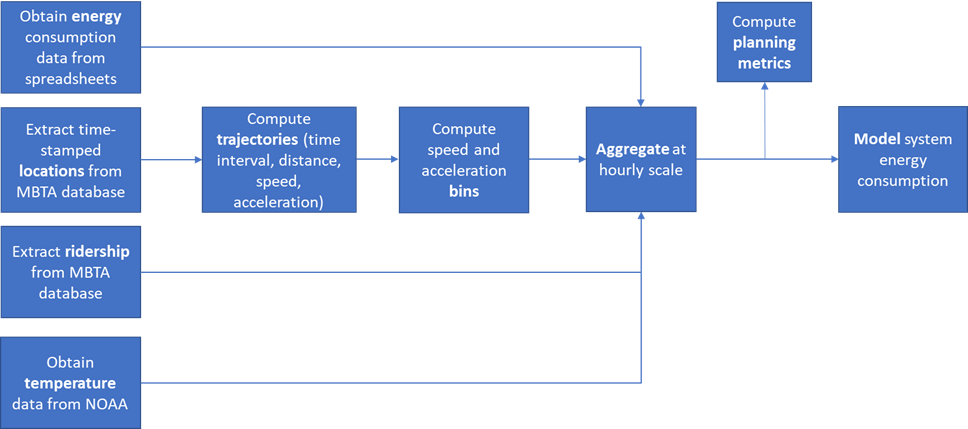
\includegraphics[scale=1]{Figure_5_Framework.png}
    \caption{Flowchart of modeling framework indicating data inputs, processing and model outputs.}
    \label{fig5}
\end{figure*}

We queried the MBTA Research Database to obtain heavy and light rail location data, along with tap-in ridership data, for a given month and year. Location data were used to compute trajectories and other train operation variables. We also obtained daily average temperature data from NOAA and spreadsheets for hourly energy consumption and monthly expenditures on electricity from the MBTA. All of these variables were then integrated into a combined table and aggregated at the desired temporal level (hourly). Using this integrated table, we created a dashboard that depicts time trends and distributions of these data as well as the trajectory per train line; see \autoref{fig6}.  The metrics of interest are: the distance traveled between observations, the time interval between observations, as well as speeds and accelerations inferred from the location and time data. The dashboard provides a visualizing platform for tracking train operation and helps us estimate the metrics. In addition, these integrated tables were used to compute planning metrics for energy, cost, and emissions. We then used these metrics as training and validation data for the estimated system energy model. 

\begin{figure*}[ht!]
    \centering
    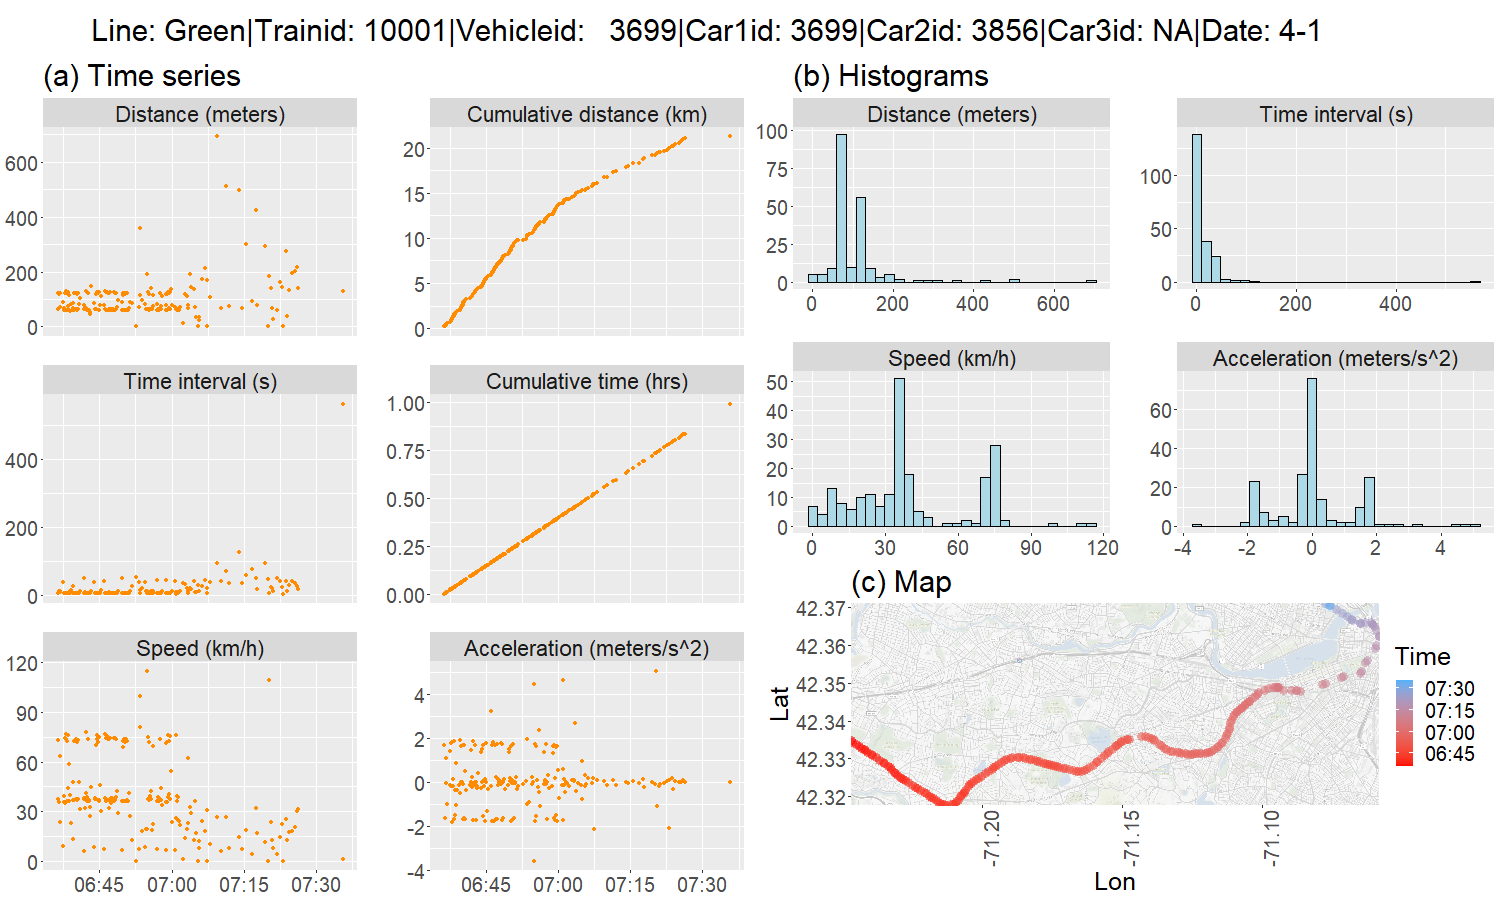
\includegraphics[scale=0.3]{Figure_6_case_green_example.png}
    \caption{Trajectory dashboard of Green line 10001 on April 1st, 2019 including a) Time series and b) histograms of vehicle distance traveled, time interval, and calculated speed per time interval, as well as c) map tracking the train location}
    \label{fig6}
\end{figure*}

The distance, time interval, speed, and acceleration for each unique train in a given day were computed using location data. Together, these measures constitute the trajectory of a given train. An example of a trajectory from the Green line is shown in \autoref{fig6}.  Based on the coordinates in the raw trajectory table, the distance traveled between each two time series records and the corresponding time interval duration were computed. Using these data, the speed, acceleration, cumulative distance, cumulative time could be calculated accordingly. All of these measurements are visualized by time series in \autoref{fig6} (a). \autoref{fig6} (b) shows the distribution of distance, time interval, speed, and acceleration observations in the form of histograms. This distribution data is important for verifying that all of the speed and acceleration measurements are plausible for the corresponding line, otherwise errors would need to be identified and addressed. Finally, \autoref{fig6} (c) presents the sequence of location (latitude, longitude) observations for a specific train on a map.  The color of each point corresponds to the time of day in order to indicate the direction that observed trains traveled over the course of the entire day.  The trajectory in \autoref{fig6} (c) is traveling from west to east because the earlier times start with red and later times end with blue.




\subsection{Speed and acceleration binning}
The energy consumption of trains fundamentally depends not only on their mass, but also on their speeds and rates of speed change (i.e., acceleration). Given the high-level system model objective, we can capture the contribution of train movement to energy consumption by observing how much time is spent at various speeds and accelerations. This allows for fewer variables (depending on how many intervals are used) and, therefore, less uncertainty in the model parameters.

To facilitate this estimation, we created equal-probability (quantile) bins for speed and acceleration.  We tested the efficacy of different bin numbers, with the objectives of parsimony and interpretability. Ultimately, we selected six bins for both speed and acceleration. These bins are summarized  in \autoref{tab:bintable}. Each bin is initially used as an indicator variable (1 or 0) for each train trajectory observation. Each indicator variable is then multiplied by the time duration of the corresponding interval in which it is observed and summed up to represent the total duration of time in a given bin. 

Based on the fundamental physics of train energy consumption \cite{wang2017electric}, both the speed and acceleration of a vehicle are contributors to the energy demand. Thus, we further compute speed-acceleration bin-time variables using each of the bins. This results in 36 combinations of speed and acceleration bins. Each interval observation is then assigned an indicator corresponding to the matching speed-acceleration bin it represents. When the data are aggregated at the hour level, the results of the speed-acceleration interaction variables denote the total time (vehicle-hours) collectively spent at a given speed interval, acceleration interval or joint speed-acceleration interval. 

For convenience, we use the notation “S[X]A[Y]” to represent the speed-acceleration interaction time variable. For example, S1A1 represents the speed-acceleration interaction time for speed bin 1 [0, 3.8 mph) and acceleration bin 1 [-5.0, -0.4 m/s\textsuperscript{2}). 


\begin{table*}[ht!]
\centering
\caption{Speed and acceleration bins}
\label{tab:bintable} \small
\rowcolors{2}{white}{gray!25}
\begin{tabular}{l l l l}
\toprule
\textbf{Bin Number} & \textbf{Percentile Range} & \textbf{Speed (miles/h)} & \textbf{Acceleration (m/s\textsuperscript{2})} \\ \midrule 
1 & {[}0, 16.7) & {[}0, 3.8) & {[}-5.0, -0.4) \\  
2 & {[}16.7, 33.3) & {[}3.8, 11.0) & {[}-0.4, 0) \\  
3 & {[}33.3, 50) & {[}11.0, 15.5) & {[}-0.1, 0) \\  
4 & {[}50, 66.7) & {[}15.5, 22.6) & {[}0, 0.1) \\  
5 & {[}66.7, 88.3) & {[}22.6, 30.1) & {[}0.1, 0.7) \\  
6 & {[}88.3, 100{]} & {[}30.1, 104{]} & {[}0.7, 5.0{]} \\ \bottomrule
\end{tabular}
\end{table*}

\subsection{Summary of variables}
Following the data processing and speed-acceleration binning, the interval observations in the dataset were aggregated at the hour level in order to reduce the number of observations. To determine how each of these variables interacts and impacts energy consumption, we estimated two models based on the observations.
The set of variables considered are summarized in \autoref{tab:variablesset}.

\begin{table*}[ht!]\small
    \centering
    \caption{Explanatory variables considered for hourly energy modeling}
    \label{tab:variablesset}
    \rowcolors{2}{white}{gray!25}
    \begin{tabular}{l p{4in}}\toprule \rowcolors{1}{gray!25}{white}
        \bf Variable & \bf Description \\\midrule
    %   Speed (miles/h)  &  train speed at each time record \\
    %   Acceleration(m/s\textsuperscript{2})  &  train acceleration at each time record \\
       Average hour speed (miles/h) & the average of all train speeds in one hour\\
       Monthly dummy & \\
       Number of trains & number of operating trains on each hour\\       
       Operating distance (vehicle-miles) & vehicle distance between each two time records\\
       Operating time (vehicle-hours) & train operating time on each hour\\
       S[X] (hours) & time spent in an equal-probability speed bin $x$ \\
       A[Y] (hours) & time spent in an equal-probability acceleration bin $y$ \\
       Ridership & tap-in ridership data for each hour\\
       Temperature (F) & average daily temperature in Boston area\\
       S[X]A[Y] (hours) & time jointly spent in speed bin S[X] and acceleration bin A[Y] summed up over all trains in the network\\
       \bottomrule
    \end{tabular}
\end{table*}

\subsection{Multiple linear regression}
A multiple linear regression (MLR) approach was used to predict hourly energy consumption as a function of the before mentioned explanatory variables. MLR has the advantage of being highly interpretable due to its simplicity, without sacrificing performance.  First, we used the Lasso technique to extract the most relevant variables. The Lasso performs this based on a regularization approach that shrinks irrelevant coefficients to zero. Following this, we then estimated a few linear regression models based on variable subsets obtained by removing further correlated variables. Multicollinearity was identified via correlation coefficients and variable inflation factors. 
The training set consisted of 80\% of the hourly observations in 2019, while the remaining 20\% was reserved for validation.
The final MLR model was selected by considering fitness and validation statistics, namely, adjusted coefficient of variation ($R^2$), root mean squared error (RMSE) and mean absolute performance error (MAPE).  Observations from the year 2020 were used to test the performance of the final model, in addition to analyzing the impacts of COVID-19.



\subsection{Random forests}
We also used a Random Forests (RF) model to predict energy consumption. Random Forests is an ensemble learning approach that estimates multiple regression trees based on respective bootstrap samples of the data \cite{ho1998random, arikan2018assessment, breiman2001random}.
It mitigates noise and bias by using a random fixed-size subset of variables at each branching (node-splitting) step of the tree partitioning process.
The two hyperparameters the modeler must select are the number of estimators (trees) and size of the subset of random features to be considered for tree partitioning. 
The goodness of fit of a Random Forests model can be determined based on error metrics computed on the out-of-bag (OOB) sample. OOB observations are those that are not present in any of the bootstrap samples. Thus, the OOB metrics serve  as an estimate of the validation error of the model. Ensemble models, such as Random Forests, are less interpretable than parametric approaches. However, in Random Forests, variable importances can be computed from the tree partitioning process. These importances can rank the relevance of each of the explanatory variables to the dependent variable.

In this application, the best hyperparameters for the RF model were 500 estimators (trees) and a random splitting-variable subset size of 40.
The entire set of 2019 hourly observations were used for training the model (noting that about 37\% of these observations are expected to be in the OOB sample). 
We reserved observations from the year 2020 for predictive performance testing. 



\section{Results and Discussion}
\subsection{Model fitness and performance}
% We estimated a linear regression (LR) model to explain hourly energy consumption. We further estimated a Random Forests (RF) model to provide validation of our variable selection in the linear model.
%The models were trained on observations from 2019. 
We gauge the fitness of the linear regression (LR) model fitness by the adjusted coefficient of determination ($R^2$), which indicates the proportion of variance explained (PVE) by the model. The RF model is evaluated by a similar PVE metric.
In determining the best parameterization for each model, we assessed the root mean squared error (RMSE) and the mean absolute percentage error (MAPE). For the LR model, these were computed on 20\% of observations in 2019 left out of the training set. In the RF model, validation metrics were computed from the out-of-bag sample observations, which are also not used by the model in training.
Finally, we compare the performance of both models on the test set of observations from the year 2020.
Based on the prediction over the year, we obtained an RMSE of 2.7 MWh and a MAPE of 4.68\% from the LR model, while the RF model resulted in an RMSE of 2.94 MWh and a MAPE of 5.01\%. 
The model fitness and performance metrics are summarized in \autoref{tab:modelmetrics}.

\autoref{fig7} shows time series of observed and predicted system-wide energy consumption. The plots indicate that the prediction errors from May to December are greater than earlier in the year, indicating that there are some temporal effects the model does not fully capture. The average residuals of linear regression is -0.31 MWh, while the average residuals of the RF one is -1.28 MWh, which proved that the distance between observation and prediction is smaller in the LR model compared with RF. Nevertheless, both models perform well in testing and are clearly robust to the COVID-19 disruptions that occurred within 2020. 

\begin{table*}[ht!]
\caption{Summary of models goodness of fit metrics. Validation metrics for the random forests model are based on the out-of-bag estimates}\small
\label{tab:modelmetrics}
\centering
\begin{tabular}{l r cc cc}
\toprule 
\bf Model & \bf Training & 
\multicolumn{2}{c}{\bf Validation} &
\multicolumn{2}{c}{\bf Test} \\
& &   RMSE (MWh) & MAPE (\%) &   RMSE (MWh) & MAPE (\%)  \\ \midrule
% Linear regression & $R^2$ & .93 & 2.70 & 4.68\% \\
% Random forests & PVE & .95 & 2.94 & 5.01\% \\
Linear regression & $R^2$: .93 & 2.19    & 3.32&2.70 & 4.68\\
Random forests    & PVE:  .95 & 1.78   & - & 2.94& 5.01\\
\bottomrule  
\end{tabular}
\end{table*}


\begin{figure*}[ht!]
    \centering
    \includegraphics[scale=0.15]{Figure_7_model_performance.png}
    \caption{Predictive performance of (a) linear regression and (b) random forests models on 2020 energy consumption for the MBTA. Residuals for both models are shown in (c)}
    \label{fig7}
\end{figure*}

\subsection{Key factors driving system energy consumption}
The coefficients estimated from the multiple linear regression model allow us to physically quantify the average effect of the relevant variables on energy consumption (summarized in \autoref{tab:MLRcoef}). The table also shows the average value for each of the variables from 2019 to provide a better sense of the magnitude of each variable and its relative contribution to the hourly energy consumption.  For reference, the average hourly energy consumption in 2019 was 47.3 MWh. Thus, we see that the intercept alone contributes a sizable net positive effect of 58.5 MWh. This could be a result of baseline operations, such as station lighting and climate control.
Temperature is next (with the linear and quadratic portions included to capture the contributions of colder and hotter temperatures). In comparison, the net effect of ridership is quite small at 0.3 MWh. This indicates that ridership is less important in predicting energy consumption compared to the train operation and climate control-related energy demands on the system.

Since it was not possible to explicitly capture the effects of third-rail heating and also due to unknown interactions with temperature, monthly dummy variables were included in the model to capture these variations. January is the baseline month. On average, there is a larger reduction in energy usage as the months proceed from March through November. The greatest savings are seen in May and October, compared to the baseline of January, when cooling and heating demands, respectively, are the lowest.

\begin{table*}[ht!]\footnotesize
\centering
\caption{Variables, estimated coefficients, p-values (based on the linear regression model), 2019 average values and contribution (product of coefficient and average value) to hourly energy consumption.}
\label{tab:MLRcoef} 
%\rowcolors{1}{white}{gray!25}
\begin{tabular}{p{.8in} l 
 >{\raggedleft\arraybackslash$}p{.7in}<{$} 
r 
 >{\raggedleft\arraybackslash$}p{.8in}<{$} 
  >{\raggedleft\arraybackslash$}p{1in}<{$} }
\toprule 
\bf {Category} & \bf {Variable} & \text{\bf Coefficient} 
& \bf {p-value} & \text{\bf 2019 Avg.} & 
\text{\bf {Contrib. (MWh)}} \\\midrule
 & Intercept & 58.48 &  $2\times10^{-16}$ &  & 58.48 \\
 & Temperature (F) & -0.81 &  $2\times10^{-16}$ & 53.5 & -43.3 \\
& Temperature$^2$(F$^2$) & 0.01 &  $2\times10^{-16}$ & 3,155.2 & 31.6 \\
 & Number of trains & 0.06 &  $2\times10^{-16}$ & 129.8 & 7.8 \\
 & Ridership & 1.49\times10^{-5} &  $3.42\times10^{-5}$ & 17,299.1 & 0.3 \\\midrule
\multirow{11}{.8in}{Monthly dummy} & February & 1.67 &  $2\times10^{-16}$ &  & 1.67 \\ 
 & March & -0.52 &  $1.18\times10^{-5}$ &  & -0.52 \\
 & April & -3.92 &  $2\times10^{-16}$ &  & -3.92 \\
 & May & -5.49 &  $2\times10^{-16}$ &  & -5.49 \\
 & June & -4.86 &  $2\times10^{-16}$ &  & -4.86 \\
 & July & -4.5 &  $2\times10^{-16}$ &  & -4.5 \\
 & August & -3.37 &  $2\times10^{-16}$ &  & -3.37 \\
 & September & -4.41 &  $2\times10^{-16}$ &  & -4.41 \\
 & October & -5.44 &  $2\times10^{-16}$ &  & -5.44 \\
 & November & -3.56 &  $2\times10^{-16}$ &  & -3.56 \\
 & December & 1.28 & $2.67\times10^{-15}$ &  & 1.28 \\\midrule 
\multirow{25}{.8in}{Speed-acceleration interaction time (hours)} & S1A1 & -0.38 & $2.33\times10^{-5}$ & 0.92 & -0.35 \\
 & S2A1 & -0.23 & 0.04 & 1.99 & -0.46 \\
 & S3A1 & 0.59 & $3.16\times10^{-7}$ & 1.623 & 0.96 \\
 & S4A1 & -0.19 & 0.13 & 1.617 & -0.31 \\
 & S5A1 & -0.81 & $7.23\times10^{-6}$ & 1.28 & -1.04 \\
 & S1A2 & 0.13 & $6.29\times10^{-8}$ & 11.27 & 1.47 \\
 & S2A2 & 0.14 & $8.15\times10^{-4}$ & 9.42 & 1.32 \\
 & S3A2 & 1.23 & $2\times10^{-16}$ & 1.57 & 1.93 \\
 & S5A2 & 0.99 & $3.74\times10^{-5}$ & 0.82 & 0.81 \\
 & S2A3 & 0.03 & $6.14\times10^{-4}$ & 10.61 & 0.32 \\
 & S3A3 & 0.27 & $1.61\times10^{-12}$ & 2.007 & 0.54 \\
 & S4A3 & 0.52 & $3.22\times10^{-8}$ & 1.07 & 0.56 \\
 & S5A3 & 0.59 & $2.2\times10^{-5}$ & 1.11 & 0.65 \\
 & S6A3 & -1.81 & $6.93\times10^{-12}$ & 0.59 & -1.07 \\
 & S2A4 & 0.02 & $4.89\times10^{-4}$ & 12.58 & 0.25 \\
 & S4A4 & -0.08 & $7.72\times10^{-3}$ & 3.49 & -0.28 \\
 & S5A4 & 0.27 & 0.06 & 3.12 & 0.84 \\
 & S6A4 & 0.88 & $4.57\times10^{-6}$ & 0.951 & 0.84 \\
 & S2A5 & 0.63 & $6.91\times10^{-5}$ & 0.954 & 0.6 \\
 & S3A5 & -0.74 & $6.23\times10^{-9}$ & 1.92 & -1.42 \\
 & S4A5 & -0.21 & 0.04 & 3.12 & -0.66 \\
 & S6A5 & 1.01 & $1.11\times10^{-9}$ & 2.11 & 2.13 \\
 & S3A6 & 2.02 & $1.4\times10^{-4}$ & 0.23 & 0.46 \\
 & S5A6 & -2.1 & $2\times10^{-16}$ & 1.46 & -3.07 \\
 & S6A6 & 0.46 & 0.01 & 2.59 & 1.19 \\ \bottomrule
\end{tabular}
\end{table*}

We also analyzed how the energy varies with the speed-acceleration interaction variables. The coefficients of these interaction variables are included in \autoref{tab:MLRcoef} and also visualized using a matrix heatmap in \autoref{fig8}. Nearly all of the interaction terms involving acceleration bin 1 (A1) have a negative coefficient except for S3A1. 
%One potential reason for this is that some trains have regenerative braking capabilities. 
The negative sign indicates a net energy saving and is reflective of those trains in the system with regenerative braking capabilities (not all of them have this technology). In contrast, a positive sign indicates a net energy consumption. We observe that the average effect of S6A5 on energy consumption is 2.13 MWh. This represents the greatest contribution to energy consumption among all positive interaction terms. These results indicate that trains spent most of their accelerating time operating within speed bin 6 (S6) and acceleration bin 5 (A5). The average hourly interaction terms effect based on 2019 measurements is 0.94 MWh.
One potential reason for the negative coefficients in positive acceleration bins (e.g.\ S3A5, S5A6) might be due to unobserved interactions that are currently not captured in the model.

\begin{figure*}[h!]
    \centering
    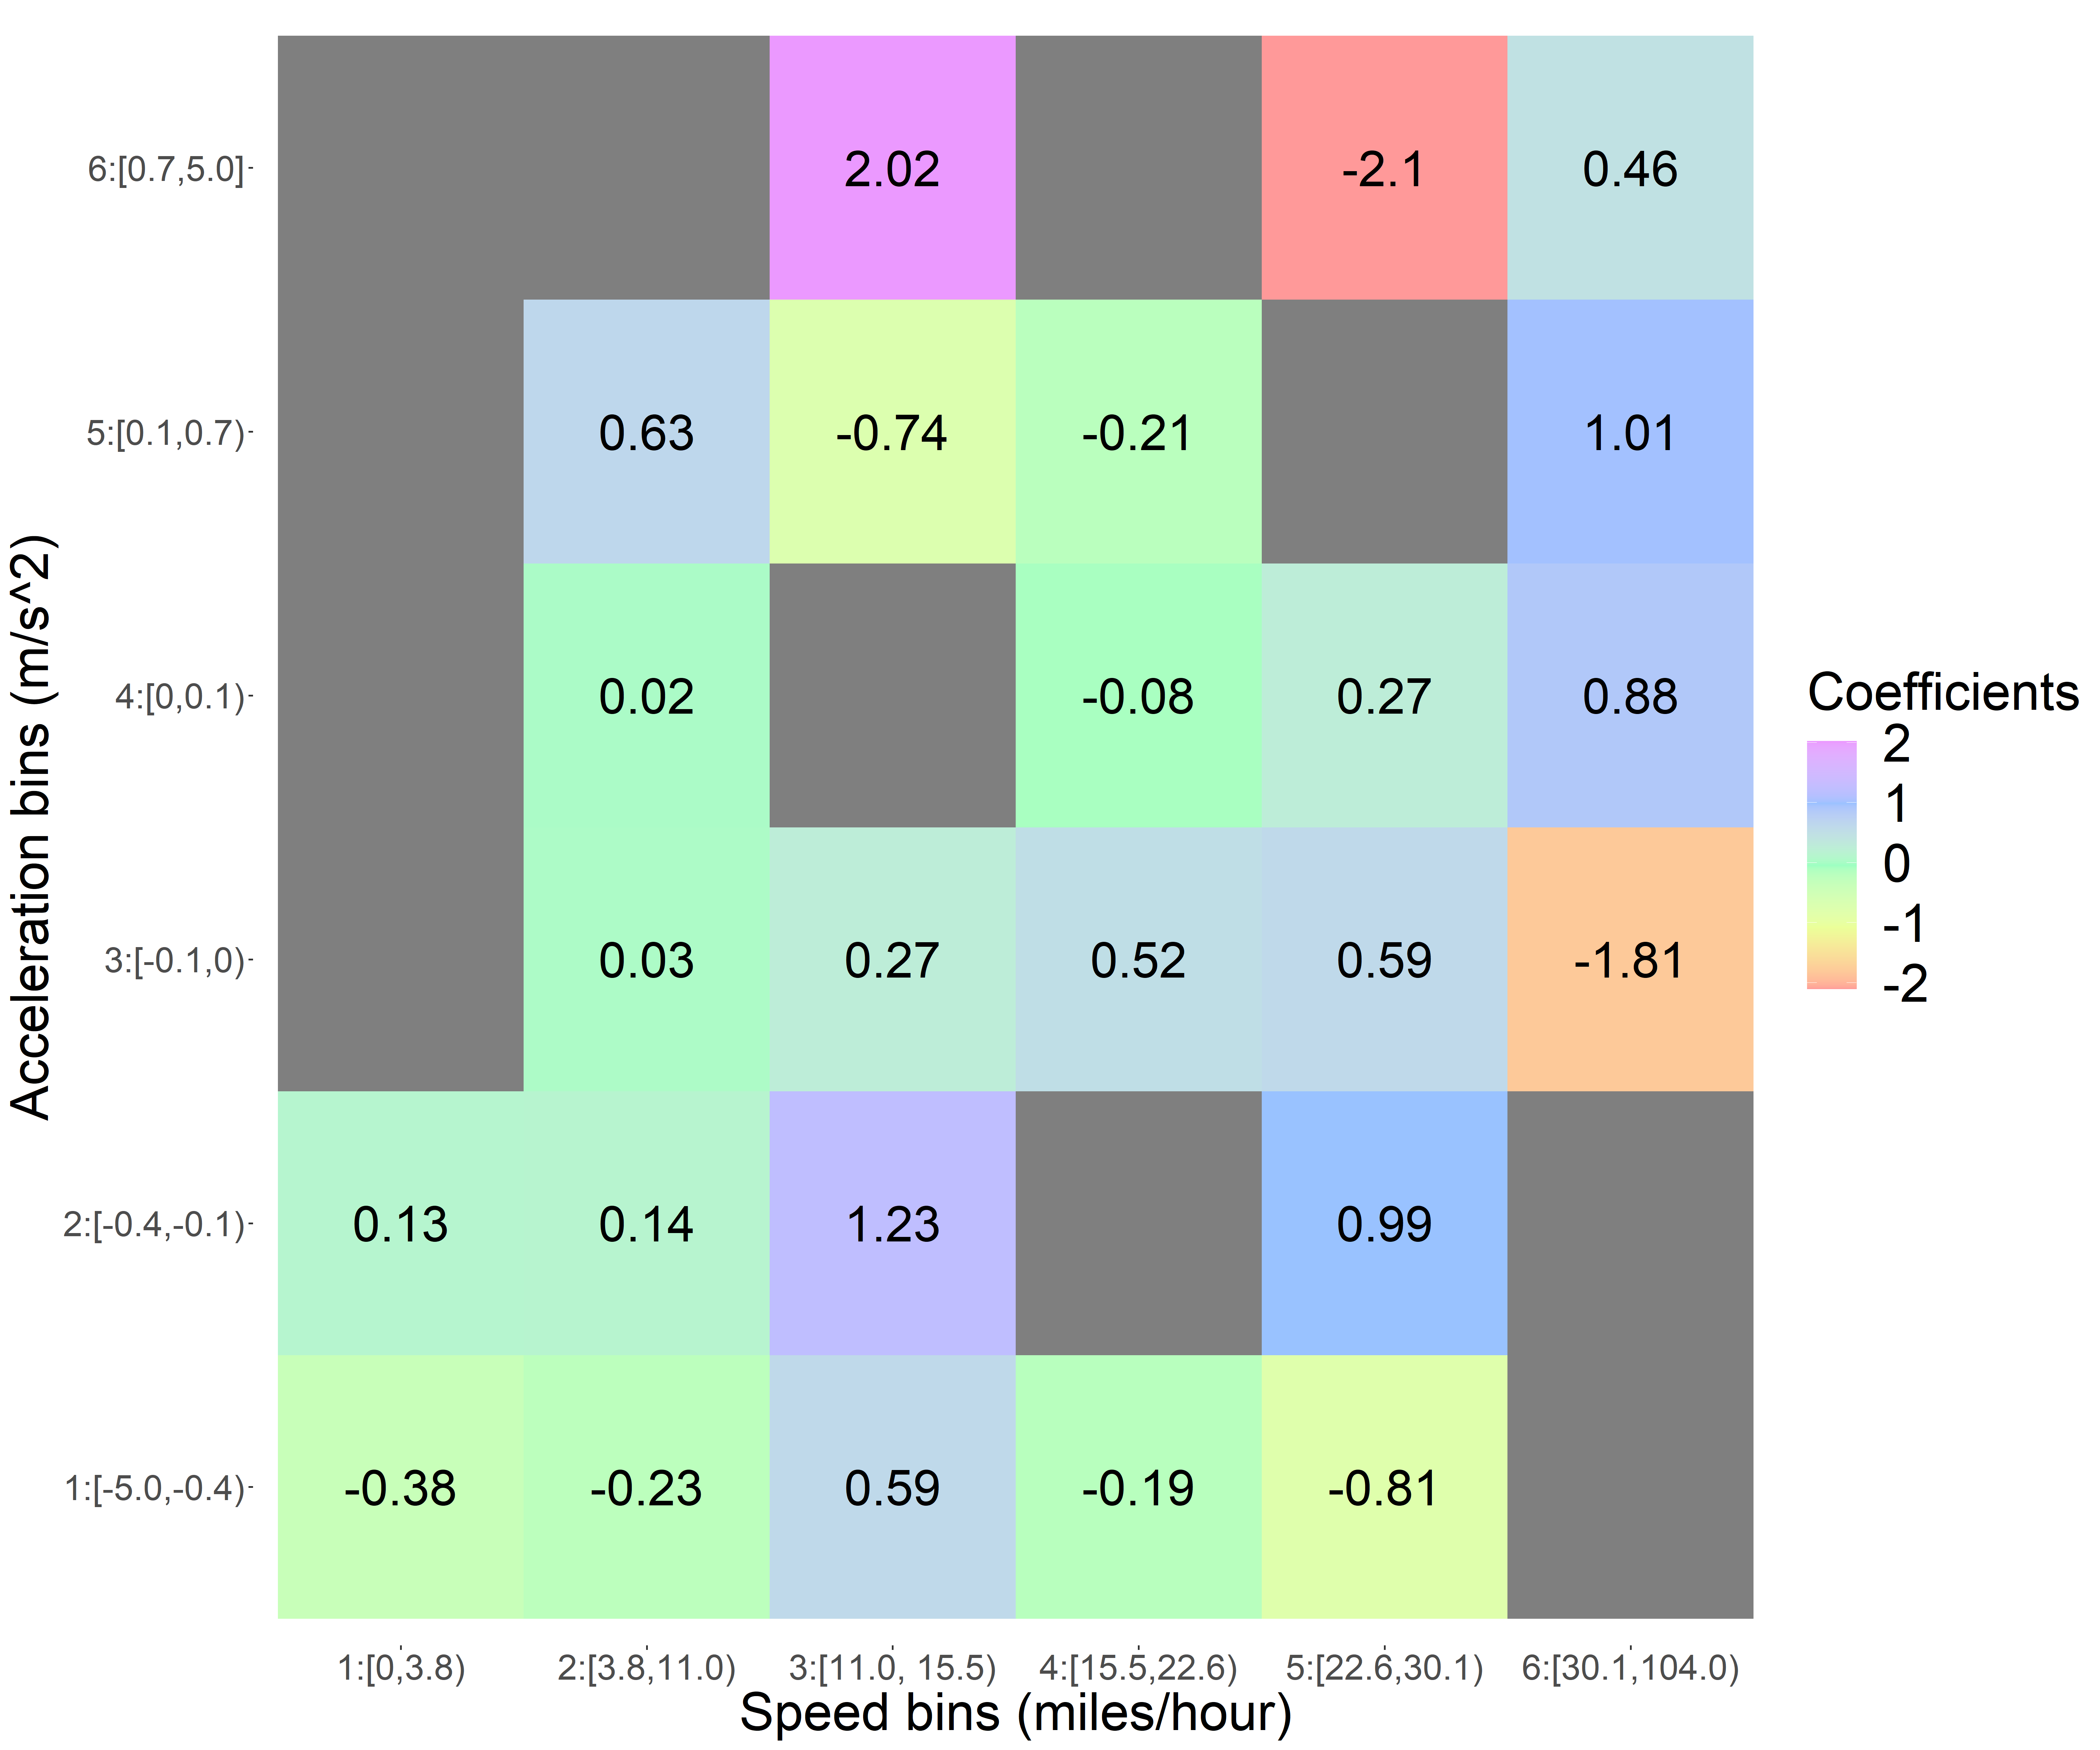
\includegraphics[scale=0.3]{Figure_8_interaction_terms_coef.png}
    \caption{Hourly energy consumption coefficients of speed and acceleration bin interaction terms. The interaction signifies the amount of time spent within a given speed interval and the corresponding acceleration interval. Negative values indicate }
    \label{fig8}
\end{figure*}

The RF model also ranks the variables based on their relevance to energy consumption (see \autoref{fig9}). Generally, we find that the importance rankings agree with the coefficients of the linear model. The number of operating trains was the variable with the greatest impact on energy consumption. In addition, average daily temperature, ridership, operating time, monthly factors and some train movements (S6A5, S5A2, S3A2) are also very important for energy consumption. This model further confirmed that trains spent most of the time operating in speed bin 6 [30.1, 104 mph) and acceleration bin 5 [0.1, 0.7 m/s\textsuperscript{2}).

\begin{figure*}[h!]
    \centering
    \includegraphics[scale=0.25]{Figure_9_RF_importance.png}
    \caption{Top 10 important variables selected by the Random Forests model. The importance is indicated by the magnitude of the ``increase in node purity" score.}
    \label{fig9}
\end{figure*}



\subsection{COVID-19 impact analysis}
COVID-19 was first reported in December 2019 and rapidly spread all over the world, reaching pandemic proportions in January 2020 \cite{cheng20202019}. It was declared a US national emergency in March 2020 \cite{2020declaring}. Subsequently,  all non-essential travel was curtailed. Public places were closed and working or schooling from home was mandated in many areas. 
Given the infectiousness of the disease, social distancing was imposed in many locales and this significantly reduced transit usage across the US \cite{liu2020impacts}.
In response to these events, and in order to cut costs as revenues declined, the MBTA reduced service on the Red, Orange and Green lines by 20\%, while reducing Blue line service by 5\% beginning March 14, 2020.
By July 2020, regular service was largely restored, even though ridership remained depressed throughout the rest of the year.


Key metrics for the MBTA urban transit system in 2019 and 2020 are compared in \autoref{tab:COVIDimpacts}. Ridership decreased by 66\% from 150.3 million tap-ins in 2019 to 51.1 million tap-ins in 2020. This ridership decline is also shown in \autoref{fig4} (b). Compared to other metrics, ridership had the greatest change (66\% decline in 2020). It did not begin to climb to prior levels until the end of 2020. 
The energy consumption in 2020 decreased by 7.6\%,  contributing to a cost decrease of 13.6\%. 
The service reductions resulted in declines in operating distance (vehicle-miles) and operating times (vehicle-hours): 5.7\% and 13.3\%, respectively. Regular MBTA rapid transit operations resumed in July 2020.


\begin{table*}[ht!]
\caption{Summary of COVID-19 impacts on MBTA. Key metrics shown %based on
for the years 2019 and 2020 and the corresponding percentage change.}\small
\label{tab:COVIDimpacts}
\centering
%\rowcolors{2}{gray!25}{white}
\begin{tabular}{lrrr}  \toprule
\textbf{Metric} & \textbf{2019} & \textbf{2020} & \textbf{ \% change} \\ \midrule
Cost ($\times 10^6$ \$) & 16.2 & 14 & $-$13.6 \\
Energy consumption (GWh) & 410.9 & 379.8 & $-$7.6 \\
Energy per vehicle-mile (kWh/mile) & 39.2 & 38.6 & $-$1.5 \\
Energy per vehicle-hour (kWh/hour) & 270.3 & 281.5 & $+$ 4.1  \\
Ridership ($\times 10^6$) & 150.3 & 51.1 & $-$66.0 \\
Vehicle-miles ($\times 10^6$) & 10.5 & 9.9 & $-$5.7 \\
Vehicle-hours ($\times 10^6$) & 1.5 & 1.3 & $-$13.3 \\
\bottomrule  
\end{tabular}
\end{table*}

\section{Conclusion}
Using data from train movement and operations, ridership, and ambient temperature, we estimated models to accurately predict and explain system-wide electricity consumption in an urban rail transit network. 
Our case study was the Massachusetts Bay Transportation Authority network, which serves the Boston metropolitan area. Notably, we developed an integrated framework for data processing and trajectory computation. We also propose a trajectory dashboard that can visualize train trajectory variables (distance, time, speed, acceleration), their distributions, and map the trajectories in real-time. 

We estimated a high-performance energy consumption multiple linear regression (MLR) model with an $R^2$ of 0.93 and random forests model (RF) with proportion of variance explained (PVE) of 0.95. Upon testing with 2020 data, these two models produced errors of less than 5.1\%. The models provide insights into the driving factors of system-wide energy consumption, while also showing potential as a decision-support tool for future planning. These key drivers were identified as: temperature, baseline energy consumption by facility, and train operations. Ridership was found to have a very small impact on energy consumption in our framework. Importantly, our model predictions held up under COVID-19 disruptions (reduced ridership and train operations).


One limitation of the current approach is that movement variables are aggregated without accounting for rail type, i.e.\ heavy or light rail. Given the clear differences in speeds and vehicle mass between these two types, the models could be improved by computing these variables (such as bin times, train numbers, etc.) as type-specific or line-specific.  Ongoing research efforts include equipping individual trains with accelerometers to calibrate physical models of electric train energy consumption using their high-resolution data. These models can then be upscaled for better system-wide energy exploration, and potentially shed more light on the contribution of ridership and other operational factors.

In addition, we plan to further develop the trajectory analysis tool into a online trajectory-energy dashboard. The dashboard can be used for real-time monitoring to pinpoint areas or vehicles in network with significant changes in energy use patterns.
Ultimately, while the models estimated have shed more light on the relevant variables for energy consumption, they would be most impactful as high-level decision-support tools that can guide planning efforts in light of future budgetary constraints or in response to disruptive events. By implementing learning procedures to map these low-level movement and operations variables to high-level planning metrics, generative processes can be estimated to produce valid synthetic data in response to any proposed policy response. Thus, future strategies can be readily assessed for energy and cost impacts and save valuable resources by providing reliable estimates to guide decision choices.

 
 
\begin{acks}
This study was undertaken as part of the Massachusetts Department of Transportation Research Program. The authors are solely responsible for the facts, the accuracy of the data and analysis, and the views presented herein. The authors would also like to thank the Massachusetts Bay Transportation Authority (MBTA) for their support and collaboration.
\end{acks}

\begin{ac}
The authors confirm contribution to the paper as follows: study conception and design: EC, EG, JO; data collection: JO, ZH; analysis and interpretation of results: EC, EG, JO, ZH; draft manuscript preparation: EC, EG, JO, ZH. All authors reviewed the results and approved the final version of the manuscript. 
\end{ac}

\begin{funding}
This research was funded by the Federal Highway Administration (FHWA) State Planning and Research (SPR) funds.
\end{funding}

\begin{das}
All the code used in generating the results and figures in this paper are publicly available at \url{}. A sample dataset is also included for reproducing the methods.
\end{das}


\subsection{References}
%\bibliographystyle{TRR}
\bibliographystyle{unsrtnat}
\bibliography{TREEM}

 

 
\end{document}
